\documentclass{article}
\usepackage[utf8]{inputenc}
\usepackage{url}
\usepackage{graphicx}
\graphicspath{{images/}}

\providecommand{\keywords}[1]
{
  \small	
  \textbf{\textit{Keywords---}} #1
}


\title{Automatic extraction of materials and properties from superconductors scientific literature}
\author{Authors}
% \date{March 2022}

\begin{document}

\maketitle

\begin{abstract}
The automatic extraction of materials and related properties from the scientific literature is getting more attention in data-driven materials science (Materials Informatics). 
We present our system for automatically extract superconductor material names and respective properties from PDF documents.
Our system combines Machine Learning and Heuristic approaches using a flexible architecture: developers can plug-in various Named Entities Recognition (NER) methods (CRF, BidLSTM, Transformers) or relation extraction approaches (ruled-based, CRF).
We have processed X papers and extracted Y materials and properties: superconducting critical temperature, crystal structure and, when available, applied pressure and measurement method.
The data obtained is suitable as input in newly material discovery projects and is available in machine-readable format.
\end{abstract}

\keywords{material informatics, superconductors, machine learning, nlp, tdm}

\section{Introduction}
% 1. Start about SC, introduce few applications (Stanev), most of SC of discovery by "feeling" or "serendipidity"
The research of new superconducting materials is still an hot topic in both fundamental science and practical applications.
Superconductors display many interesting quantum phenomena including persistent electrical currents, zero-resistivity, ability to host a strong magnetic field, vortex pinning, and quantisation of the magnetic flux. [add references]
Moreover, there is a growing list of practical and theoretical applications of superconductors including medical instruments (MRI/MNR), high-speed trains, quantum computers, and components of particles accelerators, such as the Linear Hadron Collider (LHC)~\cite{PhilippeBook, Kizu2010ConstructionOT, Cardani2017NewAO}.
However, discovering a new superconductor is still a challenging task~\cite{PhysRevB.103.014509, doi:10.1088/1468-6996/16/3/033503} because the phenomena is not yet fully understood and the relation between superconductivity and chemical composition remains unclear. 
Most of the superconductors materials have been discovered using the "feeling" (or "serendipity") approach following researchers intuition rather than any particular methodology.~\cite{doi:10.1080/08957959.2019.1695253}

% 2. Use of data-driven approaches is becoming more popular and fundamental for material discovery (there are many reviews - example citations data from Pedro) 
% ~\cite{stanev_machine_2017, le2020critical,Hamlin2019SuperconductivityNR}.(Superdocutivity releated citations)

% Pedro
In the recent years, with the creation of computational databases, such as the MaterialsProject (MP)\cite{materialsprojectJain2013} and the Open Quantum Materials Database (OQMD)\cite{oqmdkirklin2015open}, and experimental data repositories such as NIMS MDR, the focus has been steadily shifting towards a data-driven design of materials. In this new paradigm, the efficient use of data to guide experiments and materials property prediction through use of machine learning methods, for example, takes the center stage. 
For example, data-driven methods have been used to search/design magnetocaloric materials\cite{Bocarsly2017,Castro2020,court2021inverse}, photocatalysts for hydrogen splitting\cite{xiong2021optimizing}, thermoeletrics\cite{iwasaki2019machine}. Furthermore, the advance of natural language processing methods for data extraction of scientific literature, also plays a key role in supporting this new paradigm. For example, Court et. al \cite{court2018auto} developed a semi-automatic system to build a dataset of magnetic materials with their Neel and Curie temperatures. 

Other work from the same authors attempted to build a model for predicting properties, e.g. magnetic and superconducting critical temperature~\cite{court_magnetic_2020}. In the specific case of superconductivity, most of data-driven works relies on a single database: SuperCon\cite{stanev_machine_2017, le2020critical,Hamlin2019SuperconductivityNR}.

In more details, SuperCon (\url{http://supercon.nims.go.jp}) is a structured database of superconductors materials and their properties, developed at the National Institute for Materials Science (NIMS) in Japan. 
At the time of writing this paper, SuperCon contains  X inorganic and Y organic materials and is the "de-facto" standard in data-driven research for superconductors materials: about 4400 articles contains the mention "\textit{supercon database}" in Google scholar. 
% One of the main problem with predicting T\textsuperscript{c} is to make reliable models which consider also non-superconducting materials or failed experiment to provide the model with the largest amount of information. Unfortunately, this is not often the case because failures and negative results are usually not reported in scientific papers.
% % I will handle this (PC) up ffrom there to line 41.

% According to~\cite{chen2020acritical}, however, predicting superconducting critical temperature T\textsubscript{c} remains a major challenge due to lack of universal theory for superconductivity and their physical models. 
% Furthermore, the absence of  structural information is "\textit{a critical gap that needs to be addressed for the development of reliable ML models}".

% Negative results are not reported - so it's very hard to create a reliable model 

% 4. Problems of supercon
% What are the current limits of SuperCon 1 from external users: data is fully manually inserted, no structure, the database contains more then 100 fields that were introduced freely 
% I want to say that the fact that supercon was built manually provided access to data in each part of the paper without limitation. While an automatic system would require different approeaches for plot/figures, tables and text. 
SuperCon is manually curated with an average update rate of 6-10 articles (corresponding to 25-30 records) every 3 months\footnote{Obtained from \url{https://dice.nims.go.jp} news feed of "2021.12.08" and "2021.09.06".}. 
The slow process makes difficult to incorporate the information from new publications in a timely manner.
In addition, such process does not guarantee 100 percent correctness: invalid formulas, typing mistakes are known by people that have worked with the data. Unfortunately the lack of feedback system did not help to improve the quality collectively. 
For example [PC can give me some examples]

From architecture prospective SuperCon employ the same design from more than 20 years ago. The schema has not changed since then and was designed to be flexible with a key-value approach where additional properties could be introduced and collected by curators.
% Since the research focus can shift back and forth on different aspects and properties of materials (e.g. results under applied pressure, measurement of critical current, study of specific phenomena) the underlying schema could accommodate such changes. 
Today, SuperCon contains as much as 175 properties but it lacks important information like the "applied pressure" (pressure applied to obtain superconductivity), which is relevant for researchers because it can change radically the nature of a material. 
% Unfortunately, SuperCon does not contain such property systematically. 
SuperCon also lacks the "measurement method" (the method used to measure the Tc) for a) characterise multiple Tc obtained from the same material and, b) allow to distinguish calculated and experimental superconductors critical temperatures. 

% 5. What are the needs? Need for a tool of methods allowing automatic extraction (both approach: general for materials or SuperCon)
In summary, there is a strong need for a tool to produce a structured database of superconductors materials in a sustainable way. 
Ideally, our goal is to have a single tool that can be customised with ease to work in several domains. Nevertheless, at this stage, we focus only on superconductors materials research. 

% 6. in this work we present X, where we did Y and obtain Z
In this work, we present our system for automatically build a structured database of superconductors materials and properties, from scientific literature. The tool is called grobid-superconductors and is a module based on grobid~\cite{GROBID}, a machine learning library to parse and structure scientific documents, a tool that support PDFs natively, a diverse set of ML architetures (CRF, Recurrent Neural Networks (RNN) based on LSTM, and transformers where the contextual embedding can be selected between BERT and SciBERT), allowing it to work with the fulltext of scientific papers, not only the abstract.
We developed grobid-superconductors and we trained using our previous work: SuperMat~\cite{foppiano2020supermat}, an corpus of annotated linked data of superconductors research articles.


% 7. what is our purpose? 
With this tool, we aim to create a database of superconductors materials and properties obtained by processing large quantities of documents. Furthermore, with the additional capabilities from grobid we expect to provide an effective curation interface which allow rapid development of a new version of SuperCon. 


We create a database of X records by processing the whole ArXiv archive of superconductors research papers (under the category cond-mat.supr-cond). 
We named this new database  SuperCon\textsubscript{2} as the evolution of SuperCon. 
This database contains X records, of which Y with pressure. ...


% 8 what makes us different from previous work 
% Grobid-superconductors supports PDFs documents natively. This means that a) the system as access to additional layout information such as superscript, subscript, bold, italic, font name, font size which can be exploited for improved accuracy. And, b) we collect the coordinates in the document of any information that is extracted from PDF document.
% This system was designed by improving a previous architecture discussed in ~\cite{foppiano2019proposal} where two main steps were designed for entity extraction and linking, respectively. 
% In addition this tool supports different ML architectures, including CRF, Recurrent Neural Networks (RNN) based on LSTM, and transformers where the contextual embedding can be selected between BERT and SciBERT. 
% We released it with an open source licence and the source code is publicly available on Github. In this way the tool development could follow the community needs as well as benefit from external contributors.  

% Contrary to all the related work mentioned before, we work with fulltext instead of abstract, which give use access to a) additional information and materials that might not be mentioned in the abstract, and b) mention to cases where the experiments recorded absence of superconductivity. 

% Our obtained database differs from SuperCon because it contains several additional properties, such as applied pressure, measurement method, crystal structure, and space groups. 
% The database also provide access to the "enhanced PDFs" where all the entities are highlighted with different colours for each type on top of the original PDF, exploiting the coordinates discussed before. 
% We believe, this features, can improve both the quality of the curations and their effectiveness. In annotation tasks (e.g. NER) it was demonstrated that visual pre-annotations were improving the task over several aspects, including time consumption and error rate~\cite{Fort2010InfluenceOP, Nvol2011SemiautomaticSA, Lingren2014EvaluatingTI}.



\section{System}

We designed the system to follow the initial proposal \cite{foppiano:hal-02870896} which lay its foundations on the Grobid library for parsing and structuring scientific documents.
Reasons why we use the grobid library: 
 - exploit layout information
 - manage already pdf encoding crap 
 - plug-in machine learning architectures 
 - open source and maintained 
 
The system ingest PDF documents and return a JSON representation of the extracted text and the identified linked entities. 
The following section provide a deeper description of the architecture. 

\subsection{Architecture}

The architecture of this system is divided into three steps: Preprocess (a) which transforms the input pdf document or text into a set of object preserving structure and layout information. Extraction (b) is an Named Entities Recognition component , and c) Linking.


\subsubsection{Preprocess}
The Preprocess transforms the input Pdf document into structured text where structure items like title, abstract, body, and annex are extracted separately. In addition, we retain also layout information such as font type, font size, superscript, subscript, bold, italic. 
This component utilise an open source tool called Grobid~\cite{GROBID} which is a specialised machine learning library for restructuring scientific in PDF format. 




\begin{figure}[ht]
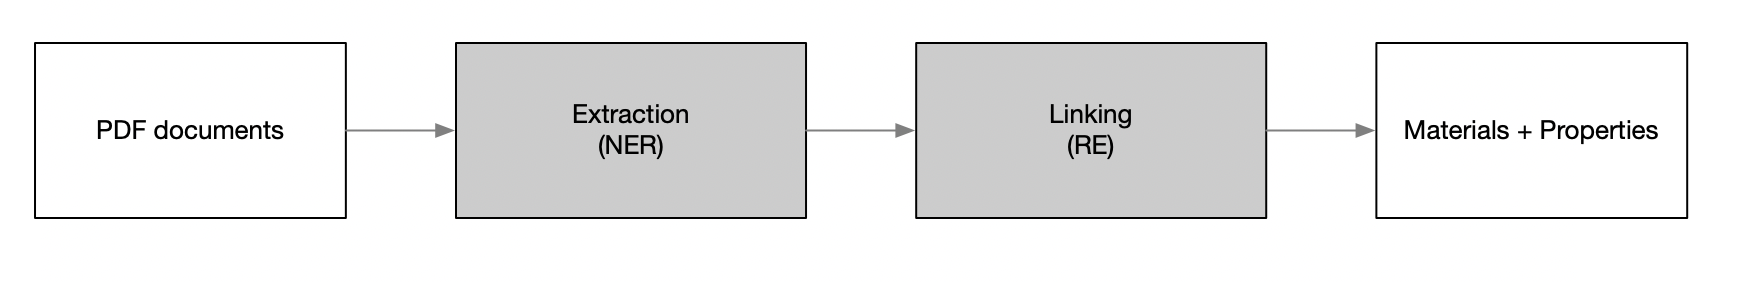
\includegraphics[width=\textwidth]{overview-schema}
\caption{Overview of the architecture}
\end{figure}

\subsubsection{Extraction}

Description of the extraction 
 - models, features etc...
 
Evaluation

Table specifies what font sizes and styles must be used for each type of text in the manuscript.

\begin{table}[ht]
\centering
\begin{tabular}{lccc}
\hline \textbf{Label} & \textbf{Precision} & \textbf{Recall} & \textbf{F1-score} \\ \hline
class           & 79.69 & 75.54 & 77.55 \\
material        & 82.9  & 81.33 & 82.1  \\
me\_method       & 82.47 & 81.26 & 81.84 \\
pressure        & 65.03 & 54.01 & 58.26 \\
tc              & 84.63 & 80.73 & 82.63 \\
tcValue         & 79.3  & 74.95 & 76.97 \\
\hline
All (micro avg) & 82.43 & 79.68 & 81.03 \\
\hline
\end{tabular}
\caption{Evaluation scores of 10-fold cross-validation using the CRF architecture. }
\end{table}


\begin{table}[ht]
\centering
\begin{tabular}{lccc}
\hline \textbf{Label} & \textbf{Precision} & \textbf{Recall} & \textbf{F1-score} \\ \hline
class           & 81.84 & 83.96 & 82.85 \\
material        & 85.18 & 83.86 & 84.51 \\
me\_method      & 83.51 & 83.37 & 83.43 \\
pressure        & 63.79 & 73.24 & 67.98 \\
tc              & 83.70 & 81.66 & 82.66 \\
tcValue         & 73.23 & 80.73 & 76.76 \\
\hline
All (micro avg) & 83.01 & 82.89 & 82.95 \\
\hline
\end{tabular}
\caption{ Evaluation scores of 10-fold cross-validation using the RNN Bid-LSTM+CRF architecture. }
\end{table}

\begin{table}[ht]
\centering
\begin{tabular}{lccc}
\hline \textbf{Label} & \textbf{Precision} & \textbf{Recall} & \textbf{F1-score} \\ \hline
class           & 79.58 & 85.79 & 82.56 \\
material        & 83.89 & 86.13 & 84.99 \\
me\_method      & 83.92 & 86.50 & 85.19 \\
pressure        & 63.92 & 71.18 & 67.27 \\
tc              & 80.91 & 83.00 & 81.94 \\
tcValue         & 76.74 & 85.00 & 80.65 \\
\hline
All (micro avg) & 83.01 & 85.06 & 83.46 \\
\hline
\end{tabular}
\caption{Evaluation scores of 10-fold cross-validation using the Transformer architecture with SciBERT. }
\end{table}

Discussion of the results 

\subsubsection{Linking}

Introduction of the linking
Objective of the linking
Algorithm in brief (three or four different scenario): 
 - only one couple of entities 
 - multiple entities:
  - general amount: linking goes by distance 
  - respectively: linking goes in order 

Evaluation

\begin{table}[ht]
\centering
\begin{tabular}{lccc}
\hline \textbf{Linked entities} (Method) & \textbf{Precision} & \textbf{Recall} & \textbf{F1-score} \\ \hline
\textbf{material-tcValue} (Rule-based)  & 88.00 	&   74.00      &	81.00      \\
\textbf{material-tcValue} (CRF)         & 68.52 &	70.11   &  69.16    \\
\textbf{tcValue-pressure} (CRF) (CRF)   & 72.92 &	67.67   &  69.76    \\
\textbf{tcValue-me\_method} (CRF)       & 49.99 &	45.21   &  44.657   \\
\hline
\end{tabular}
\caption{Evaluation scores of the linking methods. }
\end{table}

Discussion on the linking, what works, what does not work 

\subsection{End to end evaluation}

What is the end 2 end evaluation? 
How the end 2 end evaluation is performed? 

Discussion of the results, which problems are currently emerging what are the prospective for the future?

\begin{table}[ht]
\centering
\begin{tabular}{lccc}
\hline \textbf{Precision} & \textbf{Recall} & \textbf{F1-score} & \textbf{Support} \\ \hline
73.86  &	66.33 &	69.90 & 597\\
\hline
\end{tabular}
\caption{End 2 end evaluation scores. }
\end{table}

\section{Supercon\textsuperscript{2}}

Introduction of the database, which data was extracted and the format 

\subsection{Ingestion workflow}

\begin{figure}[ht]
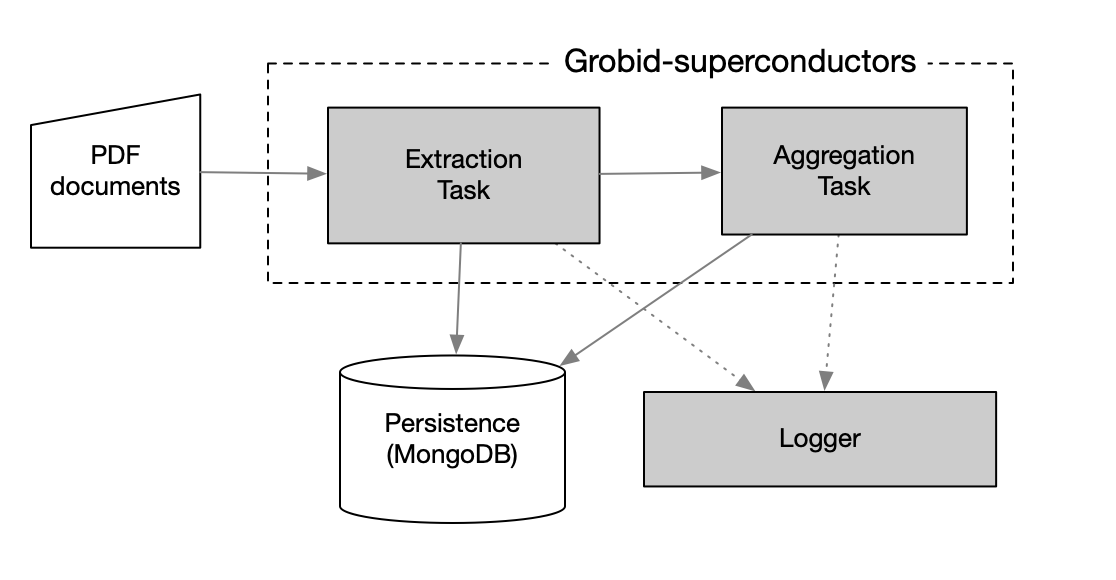
\includegraphics[width=\textwidth]{workflow-schema-1}
\caption{Schema of the ingestion workflow}
\end{figure}


Quickly discussion on the ingestion workflow 


\subsection{User interface}


\section{Conclusion}

\bibliography{bibliography}
\bibliographystyle{plain}


\end{document}
